% Genenrated by DeepSeek with minor changes

\documentclass{standalone}
\usepackage{tikz}
\usepackage{pgfplots}
\usetikzlibrary{calc}

\begin{document}

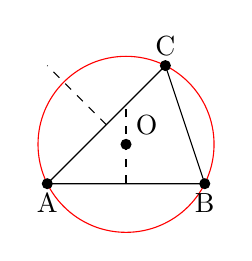
\begin{tikzpicture}

    % 定义三个点 A, B, C
    \coordinate (A) at (0, 0);
    \coordinate (B) at (2, 0);
    \coordinate (C) at (1.5, 1.5);

    % 计算垂直平分线
    % 1. AB 的垂直平分线
    \coordinate (ABmid) at ($(A)!0.5!(B)$); % AB 的中点
    \coordinate (ABperp) at ($(ABmid)!1!90:(B)$); % AB 的垂直方向点

    % 2. AC 的垂直平分线
    \coordinate (ACmid) at ($(A)!0.5!(C)$); % AC 的中点
    \coordinate (ACperp) at ($(ACmid)!1!90:(C)$); % AC 的垂直方向点

    % 计算两条垂直平分线的交点(圆心)
    \coordinate (O) at (intersection of ABmid--ABperp and ACmid--ACperp);

    % 计算半径(圆心到点 A 的距离)
    \pgfpointdiff{\pgfpointanchor{A}{center}}{\pgfpointanchor{O}{center}}
    \makeatletter
    \pgfmathsetmacro{\radius}{veclen(\pgf@x,\pgf@y)/28.45274} % pt 转换为 cm
    \makeatother

    % 绘制圆
    \draw[red] (O) circle (\radius);

    % 绘制点
    \fill (A) circle (2pt) node[below] {A};
    \fill (B) circle (2pt) node[below] {B};
    \fill (C) circle (2pt) node[above] {C};
    \fill (O) circle (2pt) node[above right] {O};

    % 可选:绘制垂直平分线
    \draw[dashed] (ABmid) -- (ABperp);
    \draw[dashed] (ACmid) -- (ACperp);

    % 可选:绘制连接线
    \draw (A) -- (B) -- (C) -- cycle;

\end{tikzpicture}

\end{document}